In Section \ref{sec:semantics} and Section \ref{sec:code_generation} we presented the semantics of Metacasanova and we showed how the meta-compiler generates the code necessary to represent the elements of the language and the evaluation of the rules expressed in terms of operational semantics. In Section \ref{subsec:code_generation_discussion} we highlighted the problem of performance degradation, due to the additional abstraction layer of the meta-compiler, and identified a possible cause in how the language manages the memory representation. For now, the memory can only be expressed with a dynamic symbol table that must be looked up at run-time in order to retrieve the value of a variable or of a class/record field. In this section we propose an extension to Metacasanova with parametric \textit{Modules} and \textit{Functors} that will allow to inline the access to record fields at compile time and to embed an arbitrary type system into the meta-type system of Metacasanova. Note that in this scope, we use the term functor with the same meaning used in the scope of the language \texttt{CamL}, i.e. a function that takes some types as input and returns a type. In order to provide additional clarity to the explanation, we introduce, in the next section, an example that we use as reference across the whole section.

\section{Case study}
Assume that we want to represent a physical body with a \texttt{Position} and a \texttt{Velocity} in a 2D space. This can be defined as a data structure containing two fields for its physical properties (the example below is written in F\#). 

\begin{lstlisting}
type PhysicalBody = {
  Position        : Vector2
  Velocity        : Vector2
}
\end{lstlisting}

In the current state of the Metacompiler, a language that wants to support such a data structure, as stated in Section \ref{sec:code_generation}, should define it either with a list of pairs $(field,value)$ or with a dictionary from .NET.

\begin{lstlisting}
Data "Record" -> List[Tuple[string, Value]] : Record
\end{lstlisting} 

Accessing the values of the fields requires to iterate through this list (or dictionary) and find the field we want to read, with two evaluation rules such as

\begin{lstlisting}
field = name
-------------
getField ((field,value) :: fields) name 
  -> value


field <> name
getField fields name -> v
-------------
getField ((field,value) :: fields) name -> v
\end{lstlisting}

\noindent
This could be done immediately by inlining the \textit{getter} (or \textit{setter}) for that field directly in the program.

In what follows we add a system of modules and functors to Metacasanova, we explain how the meta-compiler generates the code for them, and we show how to use them to improve the performance of the example above.

\section{Using Modules and Functors in Metacasanova}
\label{subsec:record_implementation}
A module definition in Metacasanova is parametric with respect to types, in the sense that a module definition might contain some type parameters, and can be instantiated by passing the specific types to use. A module can contain the definition of data structures, functions, or functors.

\begin{lstlisting}
Module "Record" : Record {
  Functor "RecordType" : * }
\end{lstlisting}

The symbol \texttt{*} reads \textit{kind} and means that the functor might return any type. Indeed the type of a record (or class) in a programming language can be ``customized'' and depends on its specific definition, thus it is not possible to know it beforehand.

We the define two modules for the \textit{getter} and \textit{setter} of a field of a record. In this example, we use type parameters in the module definitions.

\begin{lstlisting}
Module "Getter" => (name : string) => (r : Record) {
  Functor "GetType" : *
  Func "get" -> (r.RecordType) : GetType }
  
Module "Setter" => (name : string) => (r : Record ) {
  Functor "SetType" : *
  Func "set" -> (r.RecordType) -> SetType : (r.RecordType) }
\end{lstlisting}

\noindent
These two modules respectively define a functor to retrieve the type of the record field, and a function to get or set its value. Note that in the function definitions \texttt{get} and \texttt{set} we are calling the functor of the \texttt{Record} module to generate the appropriate type for the signature. This is allowed, since the result of a functor is indeed a type.

A record meta-type (i.e. its representation at meta-language level) is recursively defined as a sequence of pairs $(field,type)$, whose termination is given by \texttt{EmptyField}. We thus define the following functors:

\begin{lstlisting}
Functor "EmptyRecord" : Record
Functor "RecordField" => string => * => Record : Record
\end{lstlisting}

\noindent
The first functor defines the end point of a record, which is simply a record without fields. The second functor defines a field as the pair mentioned above followed by other field definitions.

Moreover, we must define two functors that are able to dynamically build the \textit{getter} and \textit{setter} for the field.

\begin{lstlisting}
Functor "GetField" => string => Record : Getter
Functor "SetField" => string => Record : Setter
\end{lstlisting}

The behaviour of functor is expressed, as for normal functions, through a rule in the meta-program. A rule that evaluates a functor returns an instantiation of a module. Note that, inside a module instantiation, it is possible to define and implement functions other than those in the module definition, i.e. the module instantiation must implement \textit{at least} all the functors and functions of the definition. For instance, the following is the type rule instantiating the module for \texttt{EmptyRecord}:

\begin{lstlisting}
-------------------
EmptyRecord => Record {

  Func "cons" : unit

  ------------------
  RecordType => unit

  ------------------
  cons -> ()

}
\end{lstlisting}

\noindent
The function \texttt{cons} defines a constructor for the record, which, in the case of an empty record, returns nothing. The module instantiation for a record field evaluates as well \texttt{RecordType}, and has a different definition and evaluation of the function \texttt{cons} (because it is constructed in a different way):

\begin{lstlisting}
------------------
RecordField name type r = Record {
  Func "cons" -> type -> r.RecordType : RecordType
  
  ---------------------------------------
  RecordType => Tuple[type,r.RecordType]
  
  -------------------
  cons x xs -> (x,xs)} 
\end{lstlisting}

\noindent
Note that the return type of \texttt{cons} is to be intended as calling \texttt{RecordType} of the current module, so as it were \\ \texttt{this.RecordType}.
The getter of a field must be able to lookup the record data structure in search of the field and generate a function to get the value from it. For this reason, the functor instantiates two separate modules, depending on the name of the field that we are currently examining.

\begin{lstlisting}[caption = Module instantiations for getters, label = code:getters]
//Rule 1
name = fieldName
thisRecord := RecordField name type r
-----------------
GetField fieldName (RecordField name type r) => Getter name thisRecord {
  GetType => type
  
  ---------------
  get (x,xs) -> x}

//Rule 2
name <> fieldName
thisRecord := RecordField name type r
------------------
GetField fieldName (RecordField name type r) => Getter name type thisRecord{
  Functor "GetAnotherField" : Getter
  
  ---------------
  GetAnotherField => GetField fieldName r
  
  GetAnotherField => g
  ---------------
  GetType => g.GetType
  
  GetAnotherField => getter
  getter.get xs -> v
  -------------------
  get (x,xs) -> v }
\end{lstlisting}

\noindent
Analogously, the setter of a field instantiates two separate modules whether the current field is the one we want to set or not.

\begin{lstlisting}[caption = Module instantiations for setters, label = code:setters]
name = lt
thisRecord := RecordField name type r
----------
SetField lt (RecordField name type r) => Setter name thisRecord{
  
  -----------------
  SetType => type
  
  -------------------
  set (x,xs) v -> (v,xs)}

name <> lt
thisRecord := RecordField name type r
------------
SetField lt (RecordField name type r) => Setter name thisRecord{
  TypeFunc "SetAnotherField" : Setter
  
  -------------------------
  SetAnotherField => SetField lt r
  
  ----------------------------
  SetType => type
  
  SetAnotherField => setter
  setter.set xs v -> xs'
  ----------------------------------
  set (x,xs) v -> (x,xs') }
\end{lstlisting}

\section{Functor result inlining}
If a premise or a conclusion contains a call to a functor, this call is evaluated at compile time, rather than at runtime. Metacasanova has been extended with an interpreter which is able to evaluate the result of the functor calls. The behaviour of the interpreter follows the same logic explained when presenting the code generation steps in Section \ref{sec:code_generation}, thus here we do not present the details for brevity. When a rule outputs the instantiation of the module, the generated code will contain only rules of the modules which conclusion contains a function (i.e. functions that output values, not functors). In this way the generated code will contain a different version of those functions depending on the instantiation parameters of the module.

We now show how to use the implementation of the records given in Section \ref{subsec:record_implementation} for the physical body presented as a case study.
The definition of the record type for the physical body is done through a functor

\begin{lstlisting}
Functor "PhysicalBodyType" : Record

EmptyRecord => empty
RecordField "Velocity" Vector2 empty => velocity
RecordField "Position" Vector2 velocity => body
--------------------------
PhysicalBodyType => body
\end{lstlisting}

This rule is evaluated at compile time by the interpreter that generates one module for each field of the \texttt{PhysicalBody}, containing the constructor. For example, for the field \texttt{Velocity} the interpreter will generate\footnote{Note that here we give a high-level representation of the generated rules that are actually directly generated as C\# code.}

\begin{lstlisting}
Func "cons" -> Vector2 -> unit : Tuple[Vector2,unit]

------------------------
cons x xs -> (x,xs)
\end{lstlisting}

This because the functor will call the evaluation rule for \texttt{RecordField} with the argument \texttt{(Recordfield "Velocity" Vector2 (EmptyRecord))}. This rule generates the function \texttt{cons} by evaluating the result of the functors\\ \texttt{EmptyRecord.RecordType} and \texttt{RecordField.RecordType}, which respectively produce \texttt{unit} and \texttt{Tuple[Vector2,unit]}.

Instantiating a physical body will just require to build a function that returns the type of the physical body, which is obtained by calling the functor \texttt{PhysicalBodyType}.

\begin{lstlisting}
Func "PhysicalBody" : PhysicalBodyType.RecordType

-----------------------
PhysicalBody -> PhysicalBodyType.cons((Vector2.Zero,(Vector2.Zero,())))
\end{lstlisting}

Defining the setter and getter of a field, requires to use the functor \texttt{GetField} to generate the appropriate getter function. After the module has been correctly generated, we can use the getter for the field. For example, in order to get the position field, we use the following function.

\begin{lstlisting}
Func "getPos" -> PhysicalBodyType : Vector2

GetField "Position" PhysicalBodyType => getter
getter.get PhysicalBody -> p
-------------------------------
getPos -> p
\end{lstlisting}

The result of the premise \texttt{GetField} will be evaluated at compile time through the code in Listing \ref{code:getters} and will instantiate a module containing the following function definition and rule.

\begin{lstlisting}
Func "get" -> Tuple[Vector2,Tuple[Vector2,unit]] : Vector2

-------------------------
get (x,xs) -> x
\end{lstlisting}

\noindent
Note that the second premise of \texttt{getPos} will immediately call the \texttt{get} generated in this step. The case of \texttt{setPos} is analogous except the setter takes an additional argument.

Reading \texttt{Velocity} analogously uses a functor call to generate a getter:

\begin{lstlisting}
Func "getVel" -> PhysicalBodyType : Vector2

GetField "Velocity" PhysicalBodyType => getter
getter.get PhysicalBody -> p
-------------------------------
getVel -> p
\end{lstlisting}

\noindent
This time the functor will generate two different functions in two separate modules. The first time the record is processed, \texttt{Rule 2} in Listing \ref{code:getters} will be activated (because the first field in the Record is \texttt{Position}). This rule will instantiate an additional module when evaluating the functor call in its premise, which in turn is able to get the \texttt{Velocity} field. The rule for \texttt{get} in the first module will contain in its premise a call to  \texttt{get} of the second module.

\begin{lstlisting}
//Code for module1
Func "get" -> Tuple[Vector2,Tuple[Vector2,unit]] : Vector2

module2.get xs -> v
-------------------------
get (x,xs) -> v

//Code for module2 generated by evaluating the functor in the premise of Rule 2
Func "get" -> Tuple[Vector2,unit] : Vector2

------------------
get (x,xs) -> x
\end{lstlisting}

We want to point out that this optimization has been presented on the specific case of records, but can be generalized for any situations where you would use a symbol table. Indeed any symbol table can be expressed with the representation above as a sequence of pair where the first item is the value of the current variable, and the second item is the continuation of the symbol table.

\section{Functor interpeter}
Here describe how the inlining process is implemented in the meta-compiler with the type function interpreter

\section{C-{}- optimization}
Show how to optimize the current C-- implementation by using functors to populate the symbol table.

\section{Casanova 2.5 optimization}
\begin{itemize}[noitemsep]
	\item Entity definition with functors.
	\item Entity traversal with functors (?)
	\item Rule update definition with functors.
	\item Evaluation.
\end{itemize}
Show how to use functors to define an entity as a Record and how to inline the getter and setter of fields in rules.

\section{Evaluation}
An extensive evaluation of Casanova implemented in Metacasanova, which we omit for brevity, can be found in \cite{DiGiacomo2017}. The implementation of Casanova operational semantics in Metacasanova is almost 5 times shorter than the corresponding F\# implementation in the hard-coded compiler. In addition to Casanova, we have implemented a subset of the C language called C-{}-. This language supports \texttt{if-then-else}, \texttt{while-loop}, and \texttt{for} statements, as well as local scoping of variables. The total length of the language definition in Metacasanova is 353 lines of code. The corresponding C\# code to implement the operational semantics of the language is 3123 lines, thus the code reduction with Metacasanova is roughly 8.84 times. For comparison, in Table \ref{tab:cmm} it is possible to see the code length to implement three different statements, both in Metacasanova and C\#. We tested C-{}- against Python by computing the average running time to compute the factorial of a number. C-{}- results to be 50 times slower than Python. This result is worse than what we obtained with Casanova, because in order to emulate the interruptible rule mechanism of Casanova in Python you must rely on coroutines that are slower than a program containing simple statements. Moreover, we tested the performance improvement of the optimization using Functors to represent records against the standard one using dynamic symbol tables. The test was run using records with a number of fields ranging from 1 to 10 and updating from 10000 to 1000000 instances of such records. In Table \ref{tab:functors}, we can see that the optimization using Functors leads to a performance increase on average of about 11 times, with peaks of 30 times. The gain increases with the number of fields, thus Functors are particularly effective for records with high number of fields. Figure \ref{fig:chart} shows a chart of the overall performance of the two techniques (the data points are taken from Table \ref{tab:functors}). The horizontal axis contains the amount of fields per record, while the vertical axis contains the number of records that are being updated. We can see that the performance of the dynamic table degrades considerably when increasing the number of fields, and that the higher the amount of records is, the steeper the curve is. On the other hand, the performance of the implementation with Functors is almost constant, regardless of the amount of fields or records that are being updated. Moreover, note that the performance of the dynamic table is improved by the fact that we are using a dictionary implemented in .NET, which can access the entries in $O(\log n)$. If the symbol table were represented as a meta-data structure in the language the performance would be even worse, since it would have to be encoded as a list of pairs with the field name and its value, and its manipulation would be affected by the evaluation rules that should implement this behaviour. Furthermore, the dynamic lookup should be done also to ensure that the types of the record fields are used consistently (for example to prevent that a record is constructed with incompatible values for its fields), while using the functors in Metacasanova embeds the type system of the language in the meta-type system, whose type safety is checked at compile-time rather than at runtime, and this contributes to further increase the performance.

\begin{table}	
	\caption{Running time with the functor optimization and the dynamic table with 10000, 100000, and 1000000 records.}
	\begin{tabular}{|c|c|c|c|}
		\hline
		\textbf{FIELDS}& \textbf{Functors (ms)}&\textbf{Dynamic Table (ms)} & \textbf{Gain}\\ \hline
		1&	1.00E-05&	5.00E-06&	0.50\\ \hline
		2&	9.00E-06&	1.30E-05&	1.44\\ \hline
		3&	9.00E-06&	2.70E-05&	3.00\\ \hline
		4&	9.00E-06&	4.50E-05&	5.00\\ \hline
		5&	9.00E-06&	7.00E-05&	7.78\\ \hline
		6&	9.00E-06&	9.90E-05&	11.00\\ \hline
		7&	9.00E-06&	1.33E-04&	14.78\\ \hline
		8&	9.00E-06&	1.75E-04&	19.44\\ \hline
		9&	9.00E-06&	2.20E-04&	24.44\\ \hline
		10&	9.00E-06&	2.70E-04&	30.00\\ \hline
		\multicolumn{2}{c|}{} & \textbf{Average gain} & 11.74\\ \cline{3-4}			
	\end{tabular}
	
	\vspace{0.15cm}
	\begin{tabular}{|c|c|c|c|}
		\hline
		\textbf{FIELDS}& \textbf{Functors (ms)}&\textbf{Dynamic Table (ms)} & \textbf{Gain}\\ \hline
		1&	9.60E-05&	6.30E-05&	0.66\\ \hline
		2&	9.40E-05&	1.59E-04&	1.69\\ \hline
		3&	9.50E-05&	3.04E-04&	3.20\\ \hline
		4&	9.60E-05&	5.03E-04&	5.24\\ \hline
		5&	9.60E-05&	7.52E-04&	7.83\\ \hline
		6&	9.60E-05&	1.05E-03&	10.95\\ \hline
		7&	9.70E-05&	1.41E-03&	14.57\\ \hline
		8&	9.80E-05&	1.82E-03&	18.59\\ \hline
		9&	9.90E-05&	2.29E-03&	23.17\\ \hline
		10&	1.00E-04&	2.81E-03&	28.05\\ \hline
		\multicolumn{2}{c|}{} & \textbf{Average gain} & 11.39\\ \cline{3-4}						
	\end{tabular}
	
	\vspace{0.15cm}
	\begin{tabular}{|c|c|c|c|}
		\hline
		\textbf{FIELDS}& \textbf{Functors (ms)}&\textbf{Dynamic Table (ms)} & \textbf{Gain}\\ \hline
		1&	9.47E-04&	7.29E-04&	0.77\\ \hline
		2&	9.51E-04&	1.78E-03&	1.87\\ \hline
		3&	9.50E-04&	3.33E-03&	3.51\\ \hline
		4&	9.60E-04&	5.43E-03&	5.66\\ \hline
		5&	9.65E-04&	8.03E-03&	8.32\\ \hline
		6&	9.71E-04&	1.11E-02&	11.44\\ \hline
		7&	9.75E-04&	1.47E-02&	15.12\\ \hline
		8&	9.82E-04&	1.89E-02&	19.28\\ \hline
		9&	9.92E-04&	2.37E-02&	23.86\\ \hline
		10&	1.00E-03&	2.87E-02&	28.62\\ \hline
		\multicolumn{2}{c|}{} & \textbf{Average gain} & 11.84\\ \cline{3-4}						
	\end{tabular}
	\label{tab:functors}
\end{table}

\begin{table}
	\centering
	\caption{Code length implementation of C-{}- and run-time performance}
	\begin{tabular}{|c|c|c|}
		\hline
		\textbf{Statement} & \textbf{Metacasanova} & \textbf{C\#}\\
		\hline
		\texttt{if-then-else} & 4 & 103 \\
		\hline
		\texttt{while} & 7 & 73 \\
		\hline
		\texttt{For} & 11 & 81\\
		\hline
	\end{tabular}
	
	\vspace{0.15cm}
	\begin{tabular}{|c|c|}
		\hline
		\textbf{C-{}-} & \textbf{Python} \\
		\hline
		1.26ms & $2.36 \cdot 10^{-2}$ms \\
		\hline
	\end{tabular}
	\label{tab:cmm}
\end{table}

\begin{figure}
	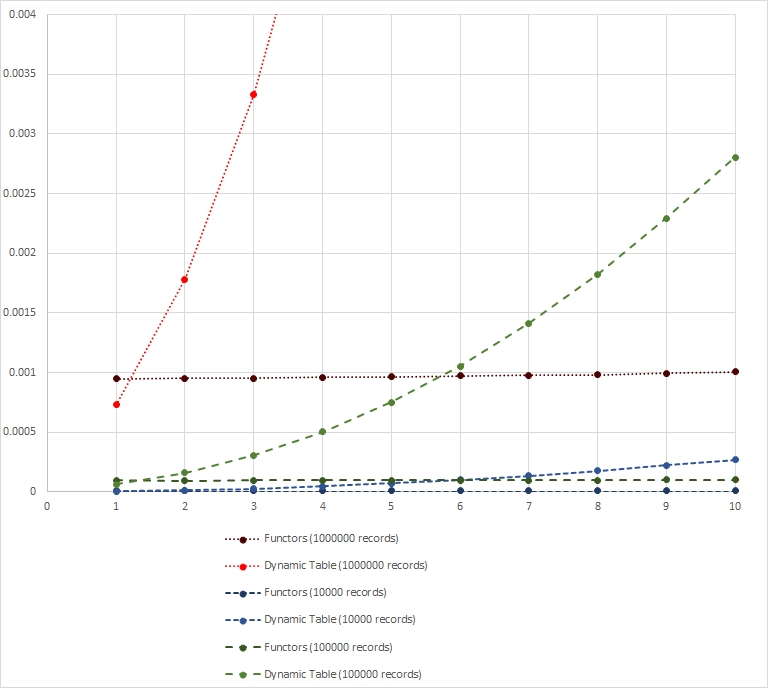
\includegraphics[width = \columnwidth]{Figures/functor_chart.jpg}
	\caption{Execution time of the different memory models}
	\label{fig:chart}
\end{figure}
